\section{研究の目的}

\begin{frame}{研究の目的}
    
    \begin{itemize}
        \item 現実の問題は非線形で,高次元・複雑→完全な数理モデルを作ることは難しい.
        \item 非線形力学システムの未来予測は一般に困難
        \begin{itemize}
            \item 特にカオスの場合は初期値鋭敏性により,(外部からの干渉も影響し)不完全な数理モデルでは予測に用いにくい.
        \end{itemize}
        \item Reservoir Computer を用いて高い精度の予測が可能
        \begin{block}{Reservoir Computer}
            内部にランダムニューラルネットワーク(Reservoir)を持つRecurrent Neural Networkの手法.Backpropagationが不必要・出力層のみの学習で計算効率が良い. 
        \end{block}    
        \item カオス時系列モデルの長期予測は生体リズムの研究に応用可能\begin{itemize}
            \item 位相シフト付きの周期外力を含む LD Cycle モデルは,外力の振幅を強めることでカオス的に振る舞う.
            \item 応用:クロニックジェットラグがシフトワーカーの生体リズムにもたらす影響についての研究など.
        \end{itemize}
    \end{itemize}      
\end{frame}

\section{先行研究}  

\begin{frame}{先行研究}
    \begin{itemize}
        \item Bollt, E. On explaining the surprising success of reservoir computing forecaster of chaos? The universal machine learning dynamical system with contrast to VAR and DMD. \textit{Chaos}, 31(1), 013108 (2021). 
            \begin{itemize}
            \item Reservior Computer による力学系時系列モデルの予測の原理に関する説明
            \item Reservior Computer と NVAR との関連
        \end{itemize}
        \item Kong, L.-W., Weng, Y., Glaz, B., Haile, M., and Lai, Y.-C. Digital twins of nonlinear dynamical systems. arXiv:2210.06144 (2022).
            \begin{itemize}
            \item 外力付き非線形力学系モデルの未来予測
            \item 外力の振幅や位相をパラメータに取ることによって biffurcation map(統計量)などを調べる.
            \item 観測されない変数がある場合も含めて,外力を実データで更新し続けた場合のcontinual forecasting を行う.
        \end{itemize}
    \end{itemize}
\end{frame}

\begin{frame}{Y. C. Lai et al. (2022) (1/3)}
    Reservior Computer は Input, Hidden, Output の三つの層から構成される.
    \begin{block}{Reservior Computer の構成:Y. C. Lai et al. (2022)}
    \vspace{0.1cm}
        \begin{minipage}{0.4\textwidth}
            \begin{figure}
                %\centering % 画像を中央揃えにする(オプション)
                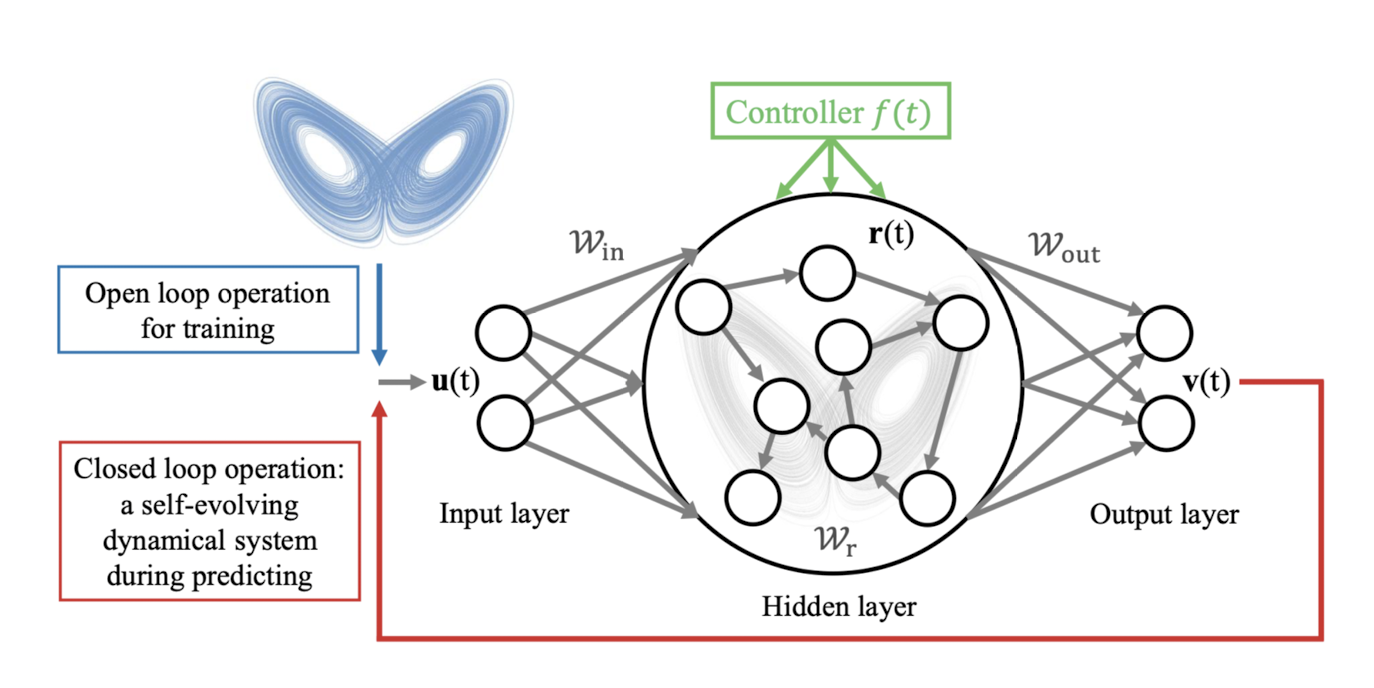
\includegraphics[width=\textwidth]{Fig/Fig.1_Lai.png}
                \caption*{Fig.1 from Y. C. Lai et al. (2022)}
                \label{Fig.1_Lai.png} % ラベルを付ける(参照する場合に使用)
            \end{figure}
        \end{minipage}%
        \begin{minipage}{0.6\textwidth}
            \begin{itemize}
                \item $\mathbf{u}(t) \in \R^{D_{\text{in}}}$: input signal. 
                \item $\mathbf{r}(t) \in \R^{D_r} $: hidden layer state vector.
                \item $f(t)$: (control) external driving signal.  
                \item $\mathcal{W}_{\text{in}} \in D_r \times D_{\text{in}}$: Weighted input matrix.  
                \item $\mathcal{W}_c$: Controller matrix.
                \item $ \mathcal{W}_r \in D_r \times D_{r}$: Weighted network matrix inside.
                \item $\mathcal{W}_{\text{out}}: D_{\text{out}} \times D_{r}$: Output weighted matrix.
            \end{itemize}
    \end{minipage}
    \end{block}
    $\mathbf{u}(t)$ に時系列モデル(low/high-dimensional Lorenz-96 climate network, driven chaotic laser systemなど),$f(t)$にはsinusoidal関数などを使用する(e.g. $f(t) = A \sin (\Omega t) + F$).
\end{frame}

\begin{frame}{Y. C. Lai et al. (2022) (2/3)}
    学習期間全体の $\mathbf{u}(t)$,全期間の $\mathbf{v}(t)$ を記録する行列をそれぞれ $\mathcal{R'}, \mathcal{V}$ とする.
    \begin{itemize}
        \item $\mathcal{W}_{\text {in }}, \mathcal{W}_c, \mathcal{W}_r$ は Reservior の学習に前もってランダムに定められる.
        \item 学習期間において,$\mathbf{u(t)}$ と $f(t)$ の実データが入力される.
        学習期間の後のself-evolving 期間では,Reservior による出力 $\mathbf{v}(t)$ と $f(t)$ の実データが予測の入力に用いられる.
        \begin{itemize}
            \item $\mathbf{r}(t)$ は 学習期間,self-evolving 期間においてそれぞれ次の式で決定される.
            \vspace{-.2cm}
            \begin{align}
                \mathbf{r}(t+\Delta t) & =(1-\alpha) \mathbf{r}(t) + \alpha \tanh \left[\mathcal{W}_r \mathbf{r}(t)+\mathcal{W}_{\text {in }} \mathbf{u}(t)+\mathcal{W}_c f(t)\right] \label{Lai_r1}\\
                \mathbf{r}(t+\Delta t) & =(1-\alpha) \mathbf{r}(t) + \alpha \tanh \left[\mathcal{W}_r \mathbf{r}(t)+\mathcal{W}_{\text {in }} \mathcal{W}_{\text {out }} \mathbf{r}^{\prime}(t)+\mathcal{W}_c f(t)\right]\label{Lai_r2}
            \end{align}
        \end{itemize}
        \item 複数の $f(t)$ に対して Reservior を sequential に学習させることで,未知の外力がある場合でも予測できるようにする.また,Hyperparameter に関する最適化を行う(後述).
        \item Reservoir に次式における$\mathcal{V}, \mathcal{R'}$ 間のLinear Regressionを通じて$\mathcal{W}_{\text {out }}$ を学習させる.
        \vspace{-.2cm}
        \begin{align}
            \mathcal{W}_{\text {out }}=\mathcal{V} \cdot \mathcal{R}^{\prime T}\left(\mathcal{R}^{\prime} \cdot \mathcal{R}^{\prime T}+\beta \mathcal{I}\right)^{-1}
        \end{align}
    \end{itemize}

\end{frame}

\begin{frame}{Y. C. Lai et al., 2022 (3/3)}
    A driven chaotic ecological system のモデル:$N$が観測できなくても予測が可能.
    \begin{minipage}{0.35\textwidth}\vspace{-1.0cm}
        \begin{align}
            & \frac{d N}{d t}=I-f(t) N P-q N \\
            & \frac{d P}{d t}=f(t) N P-P\\
            & f(t)=A \sin \left(\omega_{\mathrm{eco}} t\right)
        \end{align}
        \vspace{-.4cm}
        \begin{itemize}
            \item $P$ (学習期間のみ)と外力 $f(t)$ を入力に短期予測.定期的に $P$ を実データで更新すれば$P, N$両方のcontiual forecastingが可能.
        \end{itemize}
    \end{minipage}
    \begin{minipage}{0.64\textwidth}
        \begin{figure}
            %\centering % 画像を中央揃えにする(オプション)
            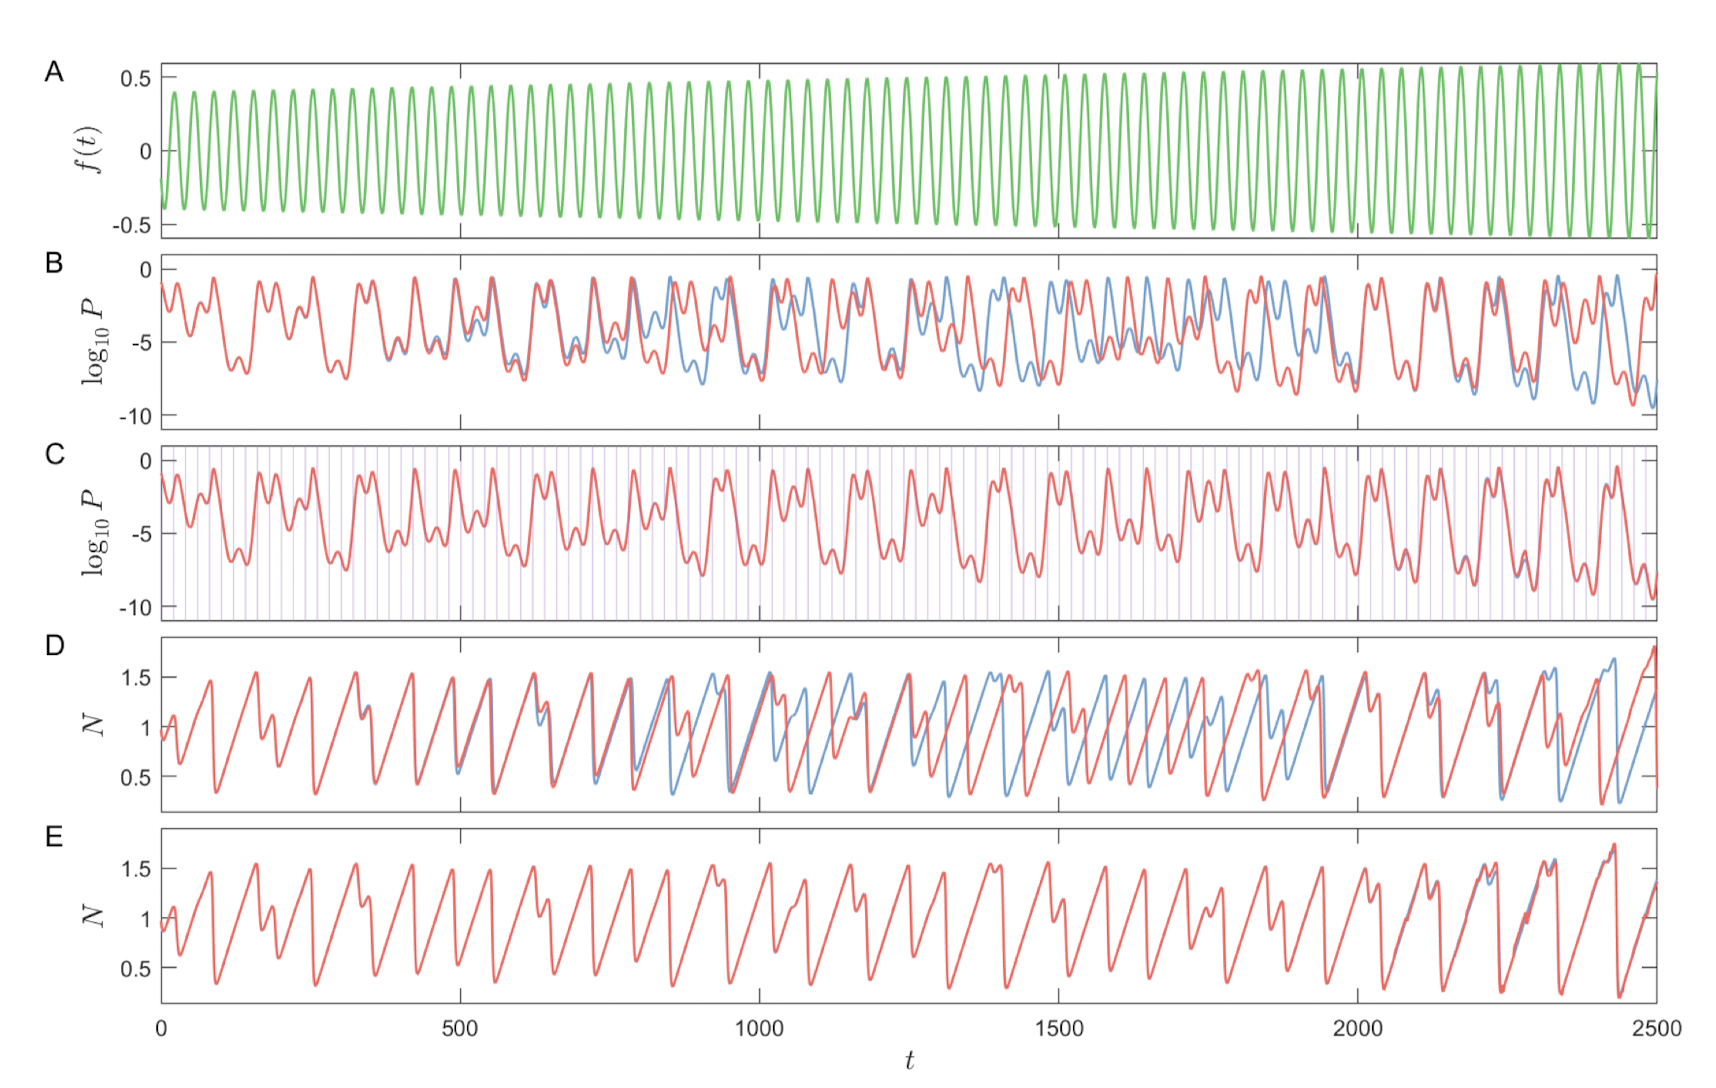
\includegraphics[width=\textwidth]{Fig/Fig.10_Lai.png}
            \caption*{Fig.10 from Y. C. Lai et al. (2022)}
            \label{Fig.10_Lai.png} % ラベルを付ける(参照する場合に使用)
        \end{figure}
    \end{minipage}
\end{frame}
